\documentclass[11pt]{report}
\title{MATH-36032 PSBC Project 2: Projectile Motion}

\setlength\parindent{0pt}

\usepackage[utf8]{inputenc}
\usepackage{amsmath}
\usepackage{amssymb}
\usepackage{amsthm}
\usepackage{listings}
\usepackage[margin=0.8in]{geometry}
\usepackage{xcolor}
\usepackage{graphicx}
\usepackage{enumerate}
\usepackage{esvect}

\usepackage{titlesec}
\titleformat{\chapter}[hang]
{\normalfont\LARGE\bfseries}{\chaptertitlename\ \thechapter.}{1em}{}

\definecolor{codegreen}{rgb}{0,0.6,0}
\definecolor{codegray}{rgb}{0.5,0.5,0.5}
\definecolor{codepurple}{rgb}{0.58,0,0.82}
\definecolor{backcolour}{rgb}{0.95,0.95,0.92}
 
\lstdefinestyle{mystyle}{
    backgroundcolor=\color{backcolour},
    commentstyle=\color{codegreen},
    keywordstyle=\color{blue},
    numberstyle=\tiny\color{codegray},
    stringstyle=\color{codepurple},
    basicstyle=\ttfamily\footnotesize,
    breakatwhitespace=false,
    breaklines=true,
    captionpos=b,
    keepspaces=true,
    numbers=left,
    numbersep=5pt,
    showspaces=false,
    showstringspaces=false,
    showtabs=false,
    tabsize=2,
    columns=fullflexible,
    numberbychapter=false
}
\usepackage{titlesec}
\renewcommand{\chaptername}{}

\titlespacing{\chapter}{-8pt}{0pt}{15pt}

\newcommand{\block}[1]{
  \underbrace{1 \cdots 1}_{#1}
}
\lstset{style=mystyle}

\makeatletter
\renewcommand*\env@matrix[1][\arraystretch]{%
  \edef\arraystretch{#1}%
  \hskip -\arraycolsep
  \let\@ifnextchar\new@ifnextchar
  \array{*\c@MaxMatrixCols c}}
\makeatother

\begin{document}

\section*{MATH-36032 PSBC Project 2: Projectile Motion}
We aim to solve two problems related to projectile motion. The projected object is a cannonball of mass $6$kg, and is fired with an initial speed of $450\text{ms}^{-1}$, at an angle $\theta$ from the ground, as shown in Figure ~\ref{fig:projectile1}.

\begin{figure}[h]
	\centering
  	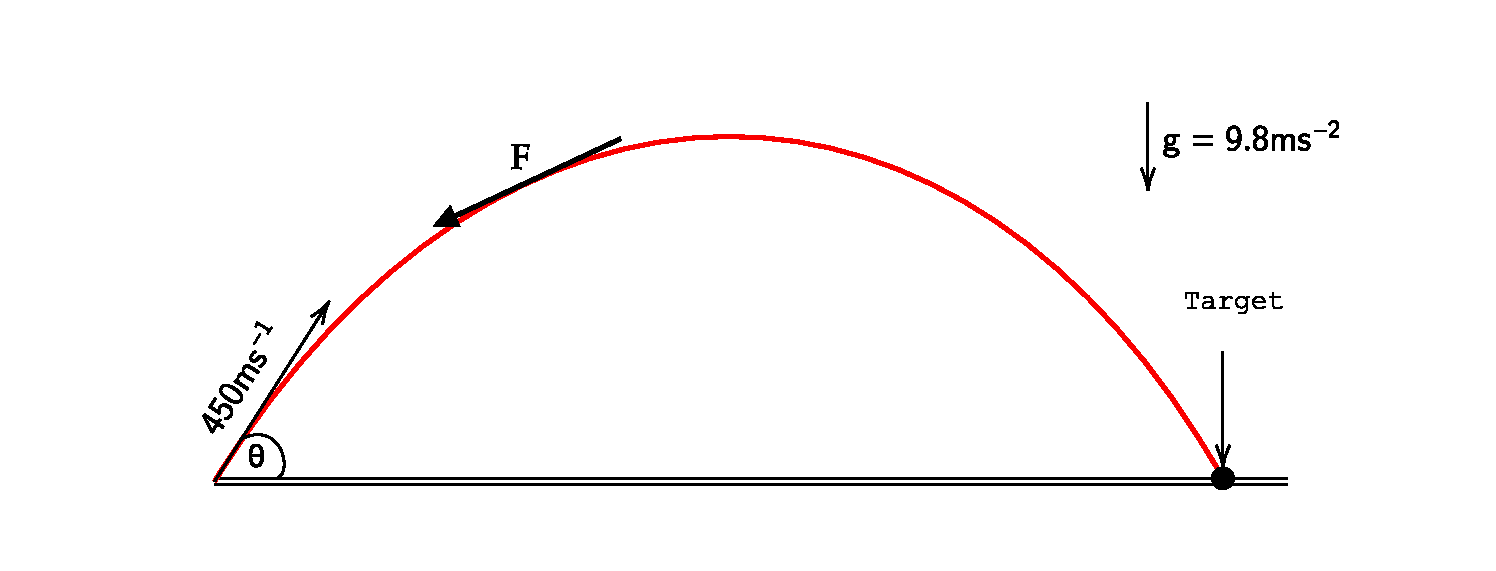
\includegraphics[scale=0.5]{assets/projectile1.eps}
  	\caption{A cannonball fired from the origin to destroy a target on the same horizontal ground.}
  	\label{fig:projectile1}
\end{figure}

We assume only the following two forces act on the cannonball:
\begin{itemize}
	\item The gravity: $\vec{g} = \begin{pmatrix} 0 \\ -9.8 \end{pmatrix}$ with gravitational constant assumed to be $9.8\text{ms}^{-2}$.
	\item The friction force: $\vec{F}=K|\vec{v}|^2$ acting in the opposite direction to the velocity $\vec{v}$ and proportional to the speed squared $|\vec{v}|^2$, with constant $K=0.00002\text{kgm}^{-1}$. Note that this can be written as $$\vec{F}=-K|\vec{v}|\vec{v}.$$
\end{itemize}

We consider Newton's Second Law of Motion to formulate a differential equation system that will model this motion.
\paragraph{Newton's Second Law of Motion} states that the sum of forces $\vec{F}$, acting on an object is equal to the mass, $m$, multiplied by the acceleration, $\vec{a}$, of the object. i.e. $$\vec{F}=m\vec{a}.$$

Let $\vec{s}(t)= \begin{pmatrix} s_x(t) \\ s_y(t) \end{pmatrix}$ be the displacement of the cannonball from the origin at a given time $t$. Since $\vec{a}=\ddot{\vec{s}}$, we can write the following using Newton's second law of motion. 

\begin{equation}
	m\dfrac{d^2 \vec{s}}{dt^2} = m\vec{g} - K|\vec{v}|\vec{v} \label{eq:n2l}.
\end{equation}

Therefore, rearranging for acceleration we have a system of second order ordinary differential equations which we can solve for $\vec{s}(t)$.
\begin{equation}
	\begin{bmatrix}[1.5]
	\ddot{s}_x(t) \\ \ddot{s}_y(t)
	\end{bmatrix}
	=
	\begin{bmatrix}[1.5]
	0 \\ -9.8
	\end{bmatrix}
	- \dfrac{K}{m}\sqrt{\dot{s}_x(t)^2 + \dot{s}_y(t)^2}
	\begin{bmatrix}[1.5]
	\dot{s}_x(t) \\ \dot{s}_y(t)
	\end{bmatrix},
	\label{eq:ode}
\end{equation}
with initial conditions expressed in terms of the initial speed and launch angle $\theta$ as
\begin{equation}
	\vec{s}(0) = \begin{pmatrix} 0 \\ 0 \end{pmatrix} \quad\text{and}\quad \dot{\vec{s}}(0) = \begin{pmatrix} 450\cos{\theta} \\ 450\sin{\theta} \end{pmatrix}.
	\label{eq:ic}
\end{equation}
Hence, we have a pair of initial value problems (IVPs) that can be solved using MATLAB.

% ******************************** Question 1 ******************************** %
\chapter{Maximum horizontal distance}
% ------ Problem ------ %
\section*{Problem}
It is known that the maximum horizontal distance can be calculated in the absence of friction force explicitly, given by the launch angle $\theta=\pi/4$.\\

In this problem we want to find the maximum horizontal distance that can be achieved for the system above with the friction force, $\vec{F}=K |\vec{v}|^2$, and the associated launch angle $\theta$.

% ------ Approach ------ %
\section{Approach}

Suppose we have a function \texttt{Distance(theta)} which returns the horizontal distance travelled by the cannonball for the given \texttt{theta}. Maximising this function for a given range of angles by using the \texttt{fminbnd} function will yield the maximum horizontal distance along with the associated angle $\theta$.

\subsection{Observations}
\paragraph{Observation I:} To implement the function \texttt{Distance(theta)} we must solve the initial value problem described by (\ref{eq:ode}) and (\ref{eq:ic}) above. This can be done by using the \texttt{ode45} solver. However, \texttt{ode45} only solves first order ODEs which are in the form $\dot{\boldsymbol{x}}=\boldsymbol{f}(t,\boldsymbol{x})$. Therefore, we must reduce the second order system into a first order system. We do this by using the following substitution:
	\begin{equation}
		\underbrace{
		\begin{bmatrix}[1.5]
			\dot{s}_1(t) \\ \dot{s}_2(t) \\ \dot{s}_3(t) \\ \dot{s}_4(t)
		\end{bmatrix}
		}_{\boldsymbol{\dot{x}}}
		=
		\underbrace{
		\begin{bmatrix}[1.5]
			{s}_2(t) \\ -\dfrac{K}{m}s_2(t)\sqrt{s_2(t)^2 + s_4(t)^2} \\ {s}_4(t) \\ -9.8 -\dfrac{K}{m}s_4(t)\sqrt{s_2(t)^2 + s_4(t)^2}
		\end{bmatrix},
		}_{\boldsymbol{f}(t,\boldsymbol{x})}
		\label{eq:ode45}
	\end{equation}
	$$\text{where}\quad s_1(t)=s_x(t), \quad s_2(t)=\dot{s}_x(t), \quad s_3(t)=s_y(t), \quad s_4(t)=\dot{s}_y(t).$$
		
	Therefore, the initial conditions become 
	\begin{equation}
		s_1(0)=0, \quad s_2(0)=450\cos{\theta}, \quad s_3(0)=0, \quad s_4(0)=450\sin{\theta}.
		\label{eq:icode45}
	\end{equation}

\paragraph{Observation II:}
The \texttt{ode45} function requires a \emph{span} (range of values for independent variable $t$) over which to find the solution. To obtain a solution for when the the cannonball reaches the ground, we require the time, $t$, it takes for the cannonball to reach the ground. However, we have no information for this exact time. \\

Instead, we consider the system when there is no resistance force $\vec{F}$ and the only force acting on the cannonball is gravity. Considering the ``SUVAT'' in the vertical component, $s_y = v_0t\sin{\theta} - \frac{1}{2}gt^2$, we can find the time when the cannonball reaches the ground by setting $s_y=0$. This gives

\begin{equation}
	t=\frac{2v_0\sin{\theta}}{g},
	\label{eq:span}
\end{equation}

where $v_0$ is the initial speed and $\theta$ is the launch angle.\\

Since air resistance works against the motion of the cannonball, it is clear that any time of flight which includes the air resistance will be lower. Hence, (\ref{eq:span}) can be used as the upper bound for the span.

\paragraph{Observation III:}
As discussed in Observation II, the span is an upper bound for the values of $t$. Therefore, the solution will have values for $t$ greater than the time taken for the cannonball to reach the ground. To avoid this, we can add an event function in the \texttt{options} argument of \texttt{ode45}. This event will simply stop solving the ODE once the cannonball touches the ground. i.e. $s_y=0$.

\paragraph{Observation IV:}
\texttt{fminbnd(f,x0,x1)} finds the \emph{minimum} value of a function \texttt{f} over the range \texttt{[x0,x1]}. However, we aim to find the maximum value of the function \texttt{Distance(theta)}. In order to achieve this we can we can use \texttt{fminbnd} on \texttt{-Distance(theta)}, i.e. the negative values for the distances, to find the maximum positive distance.

% ------ Implementation ------ %
\section{Implementation}
First, we implement a function called \texttt{Projectile(theta)}, which solves initial value problem described in (\ref{eq:ode45}) and (\ref{eq:icode45}) for a given \texttt{theta} using \texttt{ode45}.

\lstinputlisting[language=Matlab, caption={Solves the IVP described in (\ref{eq:ode45}) and (\ref{eq:icode45}).},label={lst:projectile}]{Projectile.m}

Furthermore, we define the events function discussed in Observation III as follows:\\

\lstinputlisting[language=Matlab, caption={\texttt{GroundEvent} function described in Observation III.}, label={lst:events}]{GroundEvent.m}


This will halt \texttt{ode45} from solving further, once the vertical displacement, $s_y=0$. Now consider the \texttt{Distance(theta)} function which calls \texttt{Projectile(theta)} and returns the horizontal distance reached by the cannonball.\\

\lstinputlisting[language=Matlab, caption={Returns the distance travelled for a given \texttt{theta}.}, label={lst:distance}]{Distance.m}

Finally, we have the function \texttt{FindMaxDistTheta} which uses \texttt{fminbnd} to find the maximum distance and the corresponding angle. This prints the maximum distance along with the launch angle in both degrees and radians.

\lstinputlisting[language=Matlab, caption={Finds the maximum distance and the associated angle.}, label={lst:findmaxdist}]{FindMaxDistTheta.m}
% ------ Results ------ %
\section{Result}
Below is the result of running \texttt{FindMaxDistTheta}:

\begin{lstlisting}
>> FindMaxDistTheta

Max horizontal distance: 19617.7676 metres
Launch angle: 0.77842 radians (5dp) | 44.60 degrees (2dp)
\end{lstlisting}
\ \\
Therefore, we can conclude that a maximum distance of 19617.77m (2dp) is achieved with a firing angle of $44.60^{\circ}$ (2dp) or equivalently 0.77842 radians (5dp). The plot of the projectile motion is depicted below.

\begin{figure}[h]
	\centering
  	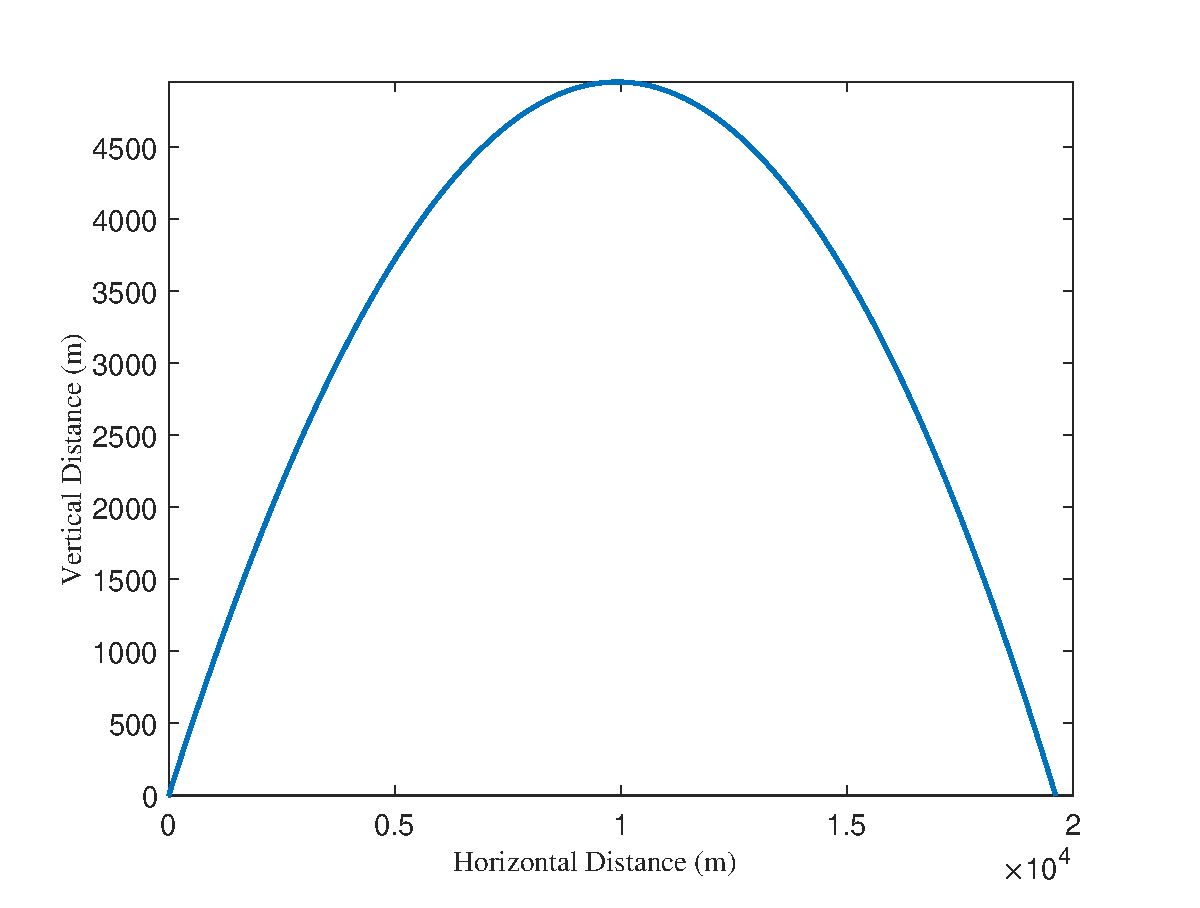
\includegraphics[scale=0.48]{assets/max_dist_plot.eps}
  	\caption{Projectile trajectory for maximum distance fired at $44.60^{\circ}$.}
  	\label{fig:plot}
\end{figure}

% ******************************** Question 2 ******************************** %
\chapter{Firing at a target}
% ------ Problem ------ %
\section*{Problem}
We wish to fire cannonballs to destroy a target at 15000 metres from the origin. However, at 12000m there are interceptors which move vertically in an attempt to block the cannonballs. Each interceptor is a 1000m long, moves vertically upwards at a constant velocity $100\text{ms}^{-1}$, and is launched every 20 seconds. Figure \ref{fig:target} shows the initial configuration at $t=0$. An interceptor is released straight away from $(12000, 0)$ as $t$ becomes greater than zero. We can conclude from the speed and the time interval that there will be a distance of 1000 metres between each interceptor because each one will travel 2000 metres before the next one is released (see Figure \ref{fig:target}). For simplicity, we assume the size of the cannonballs and the interceptors is negligible.\\

The aim is to find all possible firing angles and their associated firing times for which we can hit the target successfully.
\begin{figure}[h]
	\centering
  	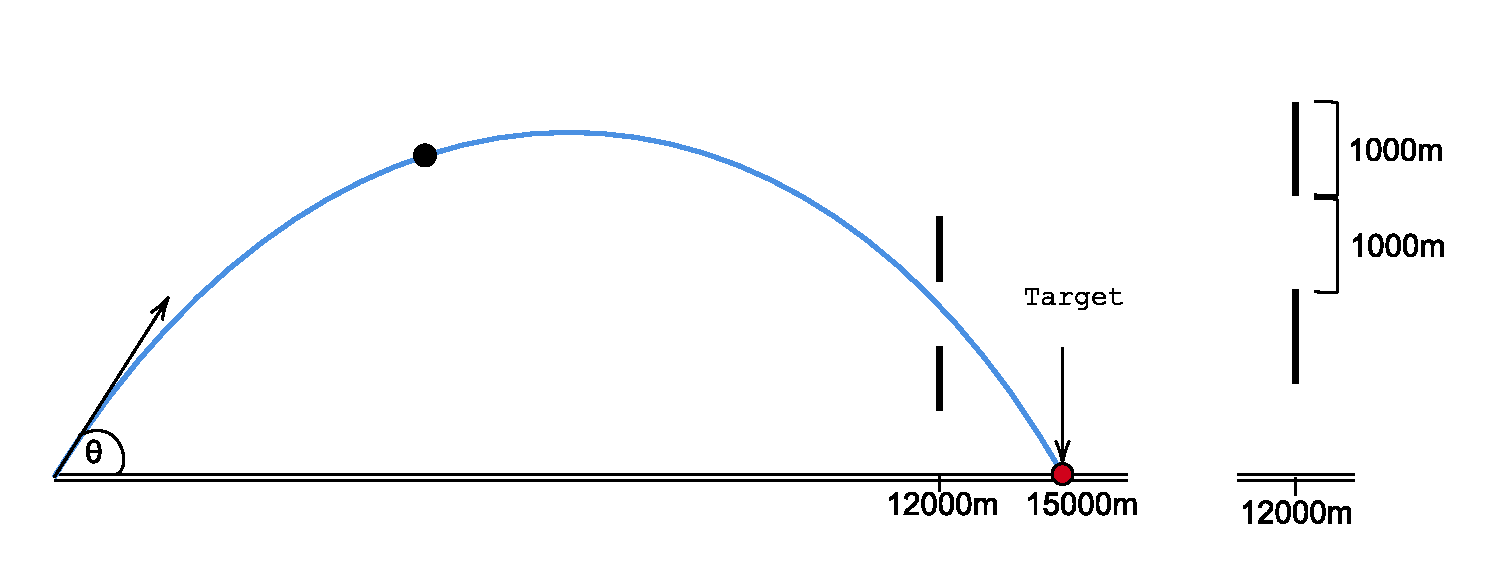
\includegraphics[scale=0.75]{assets/target.eps}
  	\caption{Setup: Fire cannons at the target avoiding the interceptors.}
  	\label{fig:target}
\end{figure}
% ------ Approach ------ %
\section{Approach}
Suppose we have a function \texttt{FiringAngles(target)}, that finds the possible firing angles for a given \texttt{target}. This can be used to obtain all the possible firing angles that will successfully hit our target. Note, that the firing angles are independent of the firing times in order to reach the target. The firing times will only be used to avoid the interceptors. \\

Now suppose, we have a function \texttt{TimeDelay(angles)}, which for a firing angle returns one time delay such that the cannonball passes the interceptor just below the interceptor. i.e. the bottom of the interceptor is at $h_{\theta}$, where $h_{\theta}$ is the height of the cannonball at distance 12000 metres from the origin, launched at angle $\theta$. \\

Combining the two functions above will allow us find the solution to the problem.

\subsection{Observations}
\paragraph{Observation I:}

In order to implement \texttt{FiringAngles(target)}, we can make use of the \texttt{fzero} function and find the angles for which \texttt{Distance(theta) - target} is equal to zero. Note that there are two firing angles that can hit a given target. To use \texttt{fzero(f,x0)}, we are required to pass in \texttt{x0} which is an initial guess (which can be a range of values). To find the appropriate initial values for each angle, we plot the following graph.

 \begin{figure}[h]
	\centering
  	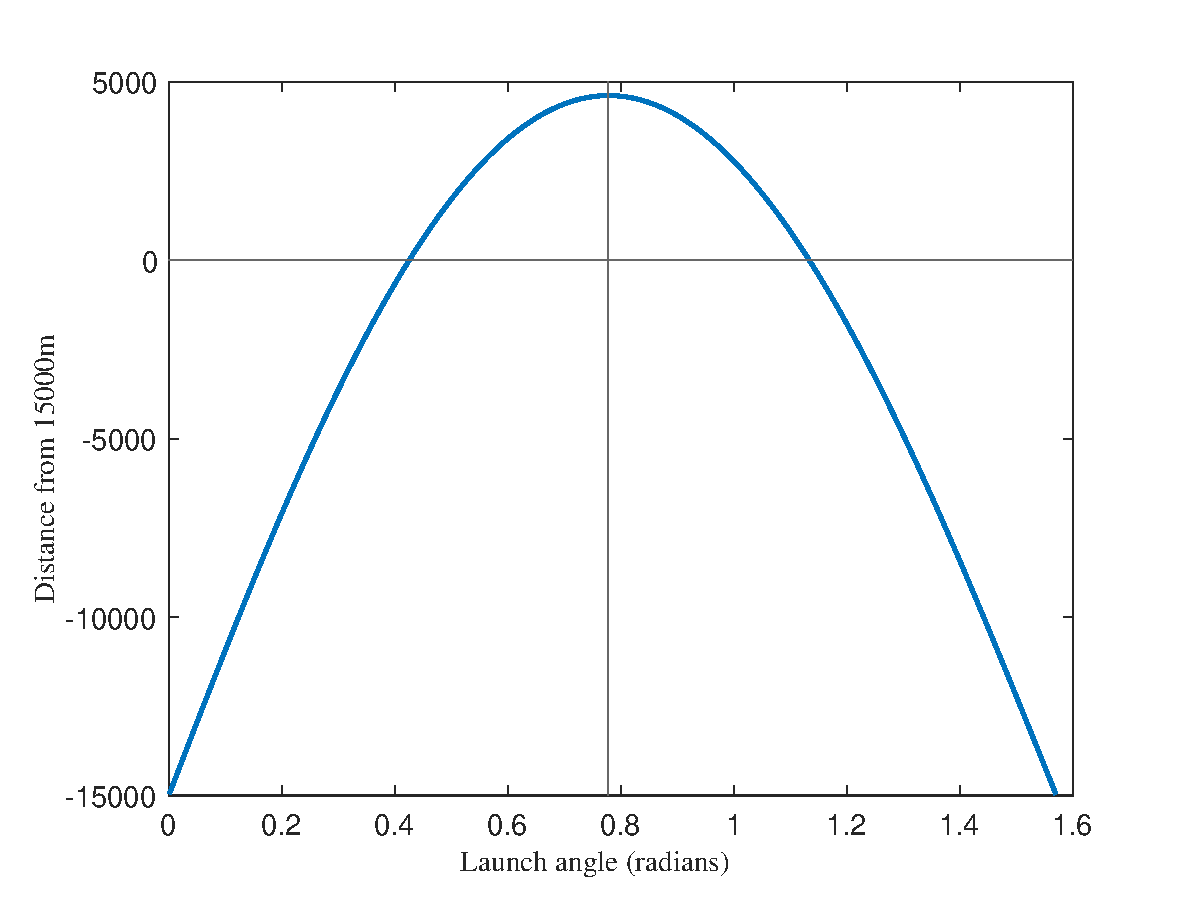
\includegraphics[scale=0.5]{assets/fzero_theta.eps}
  	\caption{Plot of \texttt{Distance(theta)-15000}}
  	\label{fig:fzero}
\end{figure}

It is clear that there are two zeros for the \texttt{theta} near 0.4 and 1.2. These are on either side of the $\text{angle}=0.77842$ (corresponding to maximum horizontal distance in part 1). Hence, we can use the initial range $(0, 0.77842)$ and $(0.77842, \pi/2)$ for the two launch angles.

\paragraph{Observation II:} The interceptors move at a constant velocity of $100\text{ms}^{-1}$. So, in 20 seconds an interceptor travels 2000 metres. Observing the setup in Figure \ref{fig:target}, we can see that the interceptors will be in the ``same'' position every 20 seconds. There is also an empty space of 1000 metres between each interceptor, which lasts for 10 seconds. \\

We want to find one time delay $t_d$ (delay after $t=0$), such that the cannonball is just below the interceptor (as mentioned earlier in the approach). The height of the point corresponding to the bottom of the first interceptor for a given time $t$, can be expressed as $$ 100t + 1000. $$\\

Now, let $h_{\theta}$ be the height of the cannonball at 12000 metres from the origin and let $t_{\theta}$ be the time it takes for the cannonball, fired at angle $\theta$, to reach this point. In order to have this height correspond to the bottom of the interceptor, we have, $$h_{\theta} \equiv 100t + 1000 \mod 2000.$$ \\

Note that we have modulo 2000, as the position of the interceptors is the same every 2000 metres travelled. This can be rearranged to $$t \equiv \frac{h_{\theta}}{100} - 10 \mod 20.$$

Since $t$ is the desired time for the cannonball to reach a distance of 12000 metres from the origin, we can take into account the time $t_{\theta}$, it takes for the cannonball to reach this distance, and calculate the time delay $t_d$ as follows, $$ t_{\theta} + t_d \equiv \frac{h_{\theta}}{100} - 10 \mod 20$$ which gives, 
\begin{equation}
	t_d \equiv \frac{h_{\theta}}{100} - t_{\theta} - 10 \mod 20.
	\label{eq:timedelay}
\end{equation} \\

Finally, we can use this time delay $t_d$, to obtain all the possible firing times. It is clear that it will take the next interceptor 10 seconds to reach $h_{\theta}$. Therefore, there is a 10 second interval $(t_d, t_d + 10)$, where the cannonball will successfully avoid hitting the interceptors. Moreover, we know that the position of the interceptors is time periodic, i.e. they are in the same position every 20 seconds. Hence, we can conclude that the time intervals where the cannonball will avoid the interceptors and hit the target successfully, are all the positive intervals $(t_d+20n, t_d+10+20n)$, where $n\in \mathbb{Z}$. 

% ------ Implementation ------ %
\section{Implementation}
First, we have the function \texttt{FindLaunchAngles(target)} which we will use to find the two possible launch angles that reach the target at 15000 metres. \\

\lstinputlisting[language=Matlab, caption={Returns the two launch angles that hit the \texttt{target}.},label={lst:launch_angle}]{FindLaunchAngles.m}
\ \\
The angles retrieved from this can be used as inputs for \texttt{TimeDelay(angles)} to find the firing times that will avoid the interceptors. However, first we implement the function \texttt{GetHeightAndDurationAt12K(theta)}, which returns the height $h_{\theta}$, and the duration $t_{\theta}$, discussed in Observation II for a given angle $\theta$. \\

\lstinputlisting[language=Matlab, caption={Returns the height and flight time at 12000m for a given \texttt{theta}.},label={lst:heightduration}]{GetHeightAndDurationAt12K.m}

Notice, in Listing \ref{lst:heightduration} we use \texttt{@InterceptorEvent} as the events function for the function \texttt{Projectile}, defined in Listing \ref{lst:projectile}. This is because, we are only concerned for a solution until the cannonball reaches a distance of 12000 metres. Hence, we can stop solving further, once this distance is reached.\\

\lstinputlisting[language=Matlab, caption={\texttt{InterceptorEvent} function.},label={lst:events2}]{InterceptorEvent.m}
\ \\
Finally, we can employ the above functions and use (\ref{eq:timedelay}) to implement \texttt{TimeDelay(angles)} which takes a list of angles as the input. \\

\lstinputlisting[language=Matlab, caption={Outputs one time delay $t_d$ each, for the given \texttt{angles}.},label={lst:timedelay}]{TimeDelay.m}

% ------ Results ------ %
\section{Result}
Let us first get the launch angles that hit the target at 15000 metres by calling \texttt{FindLaunchAngles(15000)}.

\begin{lstlisting}[title={Firing Angles (in radians) to hit target at 15000m.}]
>> [angle1, angle2] = FindLaunchAngles(15000)
angle1 = 0.425365590820470
angle2 = 1.133637131950522
\end{lstlisting}

\ \\
Now, we can use each angle and find the firing times for each angle by calling \texttt{TimeDelay} as follows:

\begin{lstlisting}[title={Time delays for both firing angles.}]
>> TimeDelay([angle1, angle2])
Time delay for angle 0.425366 = 11.280544
Time delay for angle 1.133637 = 18.171079
\end{lstlisting}

From this, we can conclude that the two launch angles that can hit the target at 15000 metres successfully are $\theta_1 = 0.425366$ and $\theta_2 = 1.133637$ (in radians). Furthermore, the respective time intervals that successfully avoid the interceptors are
 $$t_{\theta_1} = (0, 1.280544) \cup \{(11.280544 + 20n, 21.280544 + 20n) \mid n \in \mathbb{N}\}$$ 
 and
 $$t_{\theta_2} = (0, 8.171079) \cup  \{(18.171079 + 20n, 28.171079 + 20n) \mid n \in \mathbb{N}\}.$$
 in seconds.
\end{document}
